\chapter{Performance and Conclusions}
\label{chapter4}
\thispagestyle{empty}

\noindent We have presented a project work on Information Security in which we tackle the matter of privacy and personal data sharing on mobile devices. In this context, we provide a tool to control how data is shared in terms of recipients and scope of use: by implementing \textit{Sticky Policies} it is possible to describe detailed and fine-grained constraints for each shared file. \textit{Sticky Policies} are metadata that sticks to the data they describe through the application of cryptographic processes, and provided that third parties are trusted and will not illicitly share personal data with others, \textit{Sticky Policies} will always travel together with the data they refer to.

To obtain data access, third parties must ask a Trusted Authority and may be subject to its examination, aimed at assessing the service reliability.

In this work, we have implemented both a data owner and a data consumer, who communicate through an Android device application; the Trusted Authority is represented by a web server in Java, which exposes the aforementioned functionalities on Java servlets.

Let us now observe the performance of the StickyPoliciesApp using the Android Profiler available within Android Studio. The Android Profiler shows CPU, memory and network usage with the passing of time, but can be used only if the Android OS version is 5.0 (Lollipop) or higher: thus, it is not possible to test the application on a concrete device and we will just show results regarding the Android emulator, with a Nexus 5X device running Android 7.0 (full details in Appendix \ref{appendixD}).

Our first experiment is very simple: we suppose Alice wants to share a very short string of data. We test the application using as input \texttt{I cheated during last exam} (which counts 5 words and 26 characters), a string so simple that it could be the data owner Social Security Number, credit card number and pin, or Netflix username and password. As we can see from Figure \ref{fig:performance-5words}, we have two network usage peaks both in download and upload (avg speed 5KB/s) which match certificate sharing between client and server, followed by a higher peak corresponding to Alice sharing her encrypted data to Bob (avg speed 20KB/s UL, 3KB/s DL) and him asking the Trusted Authority to be granted access.

\begin{figure}
	\centering
	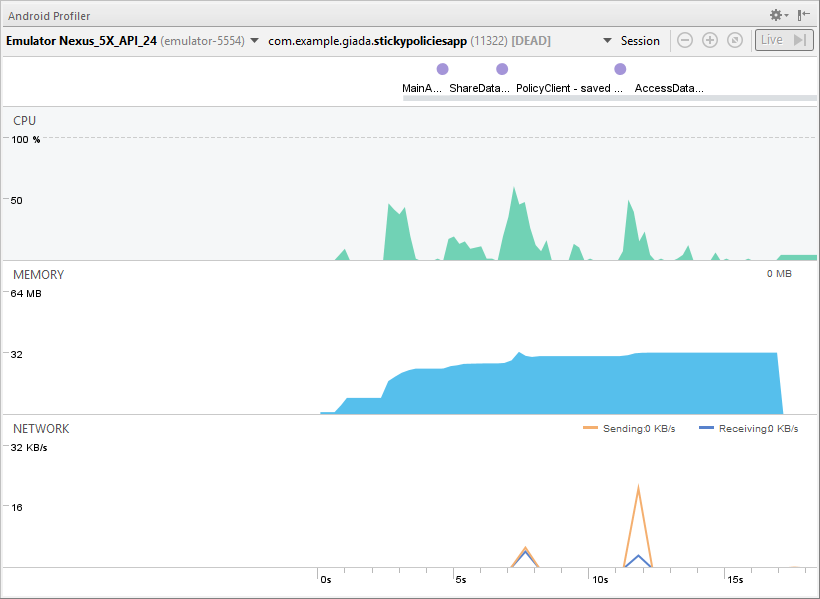
\includegraphics[width=0.95\linewidth]{Performance-5words.png}
	\caption{StickyPoliciesApp test with 5 words processing.}
	\label{fig:performance-5words}
\end{figure}

For what concerns CPU usage, we have three main peaks of duration lower than a second and occupation between 30\% and 50\%. The memory is mainly allocated for code and java usage, and it goes from 9MB at the instantiation of \texttt{MainActivity} to 32MB when \texttt{AccessDataActivity} terminates.

Next, we slightly increase the difficulty of the experiment, sharing a text document of 101 words and 605 characters. Network usage is equally divided in two moments of comparable magnitude: approximately 5KB/s in DL and UL followed by 17KB/s in UL and 2KB/s in DL. Memory usage has increased of about 10MB from the previous experiment, similarly divided between Java and code memory usage. CPU bursts have increased in number, but the percentage is usually around 25\% and the timespan of each burst is approximately 10 ms long; three main bursts are still present. Graphs from the Android Profiler are shown in Figure \ref{fig:performance-100words}.

Finally, we share a text with 1000 words (for a total count of 6804 characters): as we can observe from Figure \ref{fig:performance-1000words}, network usage radically increases, transmitting up to 91.8KB/s UL, 4KB/s DL when sharing data between Alice and Bob - this communication takes about 20 ms. Memory usage increases linearly, starting from 20MB at the instantiation to 37MB when the last activity stops. We can observe also more frequent CPU bursts: on average, the intensity has little increase in percentage, but the highest peaks reach up to 60\% even though they last less than a second.

A different approach involves changing the length of the attached \textit{Sticky Policy}, which also affects a different type of cryptography and communication. Up to now, tests have involved a basic policy with a single constraint for the shared data, for a total of 44 words, 799 characters, 849 bytes. We thus test the app performance with a more complex policy (89 words, 1527 characters, 1633 bytes), and report our findings. For these trials, we will use the same sample texts as the previous three experiments. Moreover, they require a minimal but fundamental update in the app: due to a limit in the \texttt{Bundle} maximum size, it is not possible to share this new policy between activities as it was implemented before. The new policy is then saved to internal storage after creation; this does not introduce any security weakness as the policy is public, and it is not accessible outside the application \texttt{Context}.

\begin{figure}
	\centering
	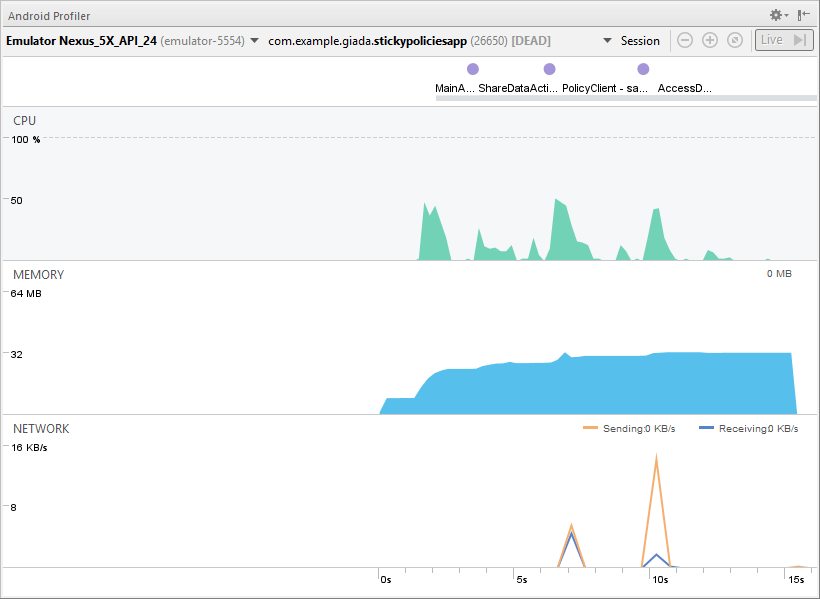
\includegraphics[width=0.95\linewidth]{Performance-5words-policy.png}
	\caption{StickyPoliciesApp test with 5 words processing and complex policy.}
	\label{fig:performance-5words-policy}
\end{figure}

From the graph in Figure \ref{fig:performance-5words-policy} we can observe that there is no significant difference with respect to the experiment with larger personal data and smaller policy. Network consumption is still divided in two main steps, the latter with a more consistent data upload; memory and CPU consumption are limited, and CPU peaks last approximately 10ms.

Increasing the size of personal data shared to 101 words, 605 characters we notice a considerable difference in network usage, in which the second transmission sends about 35KB/s and receives about 5KB/s. While memory usage is similar to the previous case, CPU usage shows an increase over time, even if with a low percentage of occupation (around 20\%), and the main three peaks (corresponding to the three major processing moments) remain unchanged between 30\% and 50\%. The graph is shown in Figure \ref{fig:performance-100words-policy}.

Finally, we test the performance with the largest input size. The graph in Figure \ref{fig:performance-1000words-policy} shows a considerable increase in network consumption, in which 95KB/s are sent in the second step; differently, memory usage is approximately the same, oscillating between 20MB to 35MB. For what concerns CPU usage, we can notice another increase both in the three major moments (percentage up to 60\%) and in the overall process, where the percentage stays below 25\%.

As a proof of concept, two additional tests were made, sharing a simple picture with a dimension of 7.05KB. In Figure \ref{fig:performance-image} the picture has been shared with the same policy as the first three experiments, while in Figure \ref{fig:performance-image-policy} we can see the results using the second policy example. Considering the whole trend of the application, we can state that there is no performance degradation depending on the data type, because both graphs are comparable to the ones seen previously. The reason for this probably lies behind cryptographic primitives processing only \texttt{byte[]}, which make a common ground between higher-level data formats.